% Chapter Template

\chapter{Introducción general} % Main chapter title

\label{INTROGEN} % Change X to a consecutive number; for referencing this chapter elsewhere, use \ref{ChapterX}

%----------------------------------------------------------------------------------------
%	SECTION 1
%----------------------------------------------------------------------------------------

La Ecología estudia las interacciones entre especies y entre ellas  y su entorno. Como rama de la Biología, tiene un desarrollado sentido de la clasificación y denomina a las de la primera clase \textit{bióticas} y \textit{abióticas} a las de la segunda. La gama de las bióticas es extensa, pero también se reduce a unas pocas categorías. En la \textit{depredación} una especie se beneficia y otra resulta perjudicada, como en el \textit{parasitismo}, mientras que en la \textit{competencia} los individuos, ya sean o no de la misma especie, disputan un mismo recurso. Estos tres tipos de relaciones se caracterizan por la realimentación negativa, resultan perjudiciales para una de las partes y beneficiosas para la otra. 

Si una de las especies obtiene beneficio pero para la otra es neutral se trata de \textit{comensalismo}. Finalmente, si la relación es positiva para ambas especies, es \textit{mutualismo}. En Ecología se contemplan estas relaciones desde un punto de vista de funcional y mecanicista \cite{rockwood2006introduction}, atendiendo sobre todo a los flujos de intercambio de materia, energía o servicios.

El conjunto de interacciones crea sistemas de gran complejidad. La dinámica de las poblaciones, puede describirse utilizando modelos matemáticos. Además, en las últimas dos décadas, la ciencia de redes ha contribuido al conocimiento de las comunidades ecológicas aplicando sus propias técnicas de análisis. Estas descripciones, fundamentadas en modelos y propiedades topológicas, son fenomenológicas \cite{van2010ethical}.

Los distintos enfoques metodológicos suponen a veces dificultades de comunicación, pero se enriquecen. En esta tesis se plantean contribuciones al estudio del \textit{mutualismo} desde el modelado matemático y la ciencia de redes, intentando no perder de vista su significado biológico.

\section{El mutualismo en ecología}

El término \textit{mutualismo} tuvo su origen en economía política a principios del XIX, relacionado con distintas concepciones utópicas. Fue el filósofo Pierre Joseph Proudhon el que hizo del mutualismo el eje de su teoría social y económica.

\enquote{\itshape [Mutualismo es] un sistema de equilibrio entre fuerzas libres, en el cual está cada una segura de gozar de los mismos derechos bajo la condición de llenar los mismos deberes, y 
de obtener las mismas ventajas a cambio de los mismos servicios} \cite{proudhon1868capacite}.

La idea de beneficio compartido fue trasladada al campo de la biología por el parasitólogo belga Pierre-Joseph van Beneden \cite{boucher1982ecology}, que escribió:

\enquote{\itshape Al lado [de los parásitos y comensales] hay otros que se prestan mutuamente servicios [..]. Creemos que es más justo llamarles Mutualistas} \cite{van1878commensaux}.

El mutualismo puede adoptar varias formas e intensidades. La característica que lo diferencia del resto de relaciones ecológicas es la cooperación entre especies mediante que intercambian servicios o bienes \cite{bronstein2001exploitation}.


%-----------------------------------
%	SUBSECTION 1
%-----------------------------------
\subsection{Tipos de mutualismo}
\label{TIPOS_DE_MUTUALISMO}
	
Las relaciones mutualistas pueden clasificarse según distintos criterios. Por el \textbf{tipo de convivencia}, se diferencia el \textit{mutualismo de simbiosis}. Las especies solo pueden vivir en una relación íntima, como las que se estableces entre numerosas especies de animales y su flora intestinal o entre bacterias y virus \cite{moran2005players}. Si, por el contrario, no hay una convivencia permanente se habla de \textit{mutualismo no simbiótico}.
	
Atendiendo a la \textbf{naturaleza del beneficio recibido}, puede ser de bienes o servicios. La polinización pertenece al primer tipo. Los animales (invertebrados en su mayoría, pero también pequeños pájaros y murciélagos) se alimentan de polen o néctar y actúan a cambio como vectores de fertilización de las plantas. La biología de la polinización es muy rica. En ocasiones, las ceras o aceites florales pueden servir para la construcción de nidos, y algunas especies de flores han desarrollado engaños para los insectos que no reciben en esa situación ningún bien a cambio \cite{rech2014biologia}.

\begin{figure}[h!]
\centering
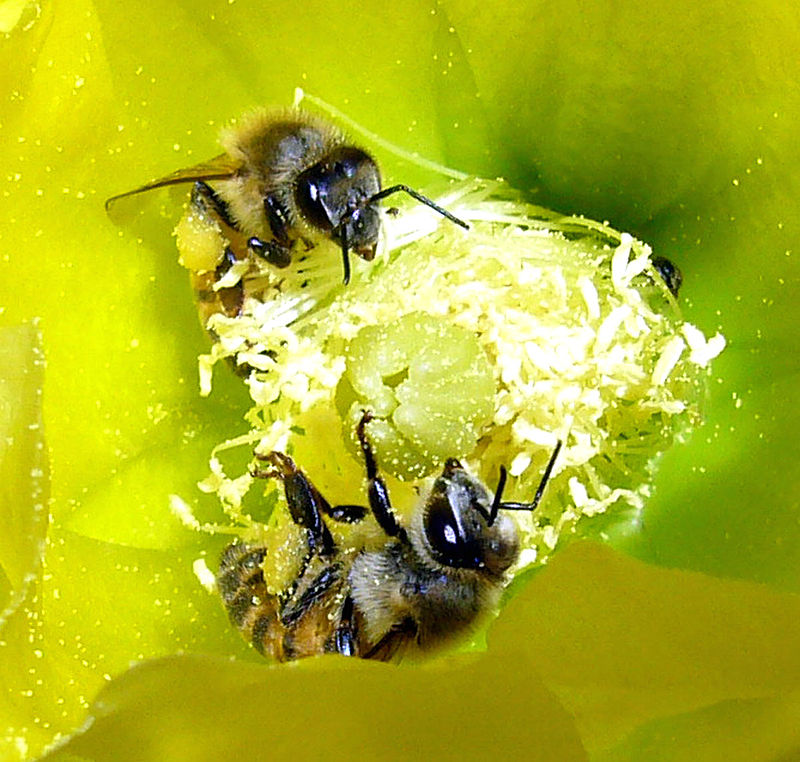
\includegraphics[scale=0.33]{Figures/INTRO_Pollination.jpg}
\caption{\textit{Apis mellifera} libando en una flor de \textit{Opuntia basilaris}, California (Estados Unidos). Fotografía de Jessie Eastland, \small{\texttt{CC BY-SA 3.0}}.}
\label{fig:INTRO_Pollination}
\end{figure}

Las comunidades de plantas y dispersores de semillas funcionan con el mismo esquema de intercambio de alimentación por servicio. Los frugívoros obtienen comida y en compensación reparten las semillas de la planta. Este tipo de mutualismo se registra sobre todo en los trópicos \cite{bascompte2007plant, estrada2012frugivores}.
	
Aunque menos comunes, también hay intercambios de recurso por recurso, como entre la bacterias del tipo \textit{Rhizobium} y las leguminosas a cuyas raíces se fijan. La bacteria proporciona nitrógeno a la planta y se alimenta de los azúcares que esta produce \cite{lindstrom2010biodiversity}.
	
Finalmente, el intercambio de servicio por servicio es la base de simbiosis como la de las anémonas con los peces y crustáceos que se han adaptado a vivir entre sus tentáculos venenoso. La anémona protege al huésped de los depredadores y a cambio este limpia sus parásitos \cite{mebs2009chemical}.

Otra distinción se basa en la \textbf{importancia vital para los actores}. En el \textit{mutualismo obligatorio} cada especie requiere del concurso de la otra para subsistir. Se suelen citar los ejemplos de yuca y sus polillas \textit(Prodixidae) o el ya citado de la anémona, aunque hay dudas de que sean absolutamente obligatorios \cite{briand1982phylogenetic, addicott1995cheating}. Está muy asociado a una gran especialización y coevolución de los mutualistas. En el \textit{mutualismo facultativo}, la relación no tiene ese carácter esencial. Es el más común en las comunidades de plantas y polinizadores \cite{geib2012tracing}.

Una última distinción se basa en la \textbf{recepción directa o indirecta del beneficio}. El \textit{mutualismo directo} es el más común, pero a veces interviene una tercera especie que
intermedia entre las dos. Boucher, James y Keeler exponen diversos ejemplos en su artículo ya citado. Desde un punto de vista de teoría de redes este \textit{mutualismo directo} es una composición de dos pares de relaciones.


\begin{figure}[h!]
\centering
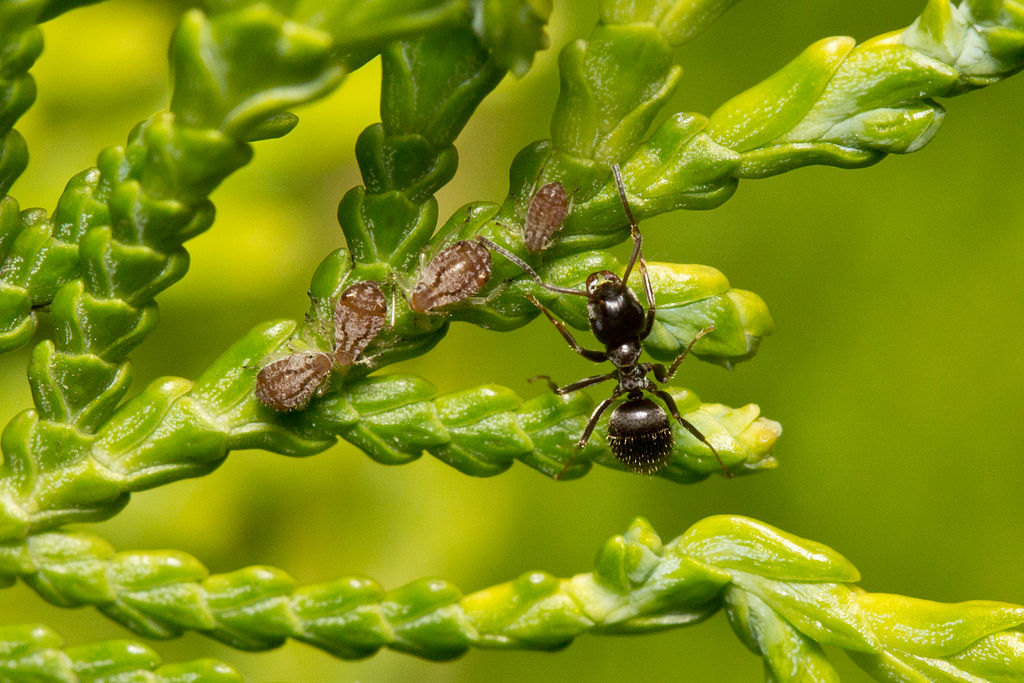
\includegraphics[scale=1]{Figures/INTRO_Lasius_niger_y_Cinara_tujafilina_en_Thuja_occidentalis.jpg}
\caption{\textit{Lasius niger} cuidando de varios ejemplares de \textit{Cinara tujafilina} sobre hojas de la conífera Tuya del Canadá \textit{Thuja occidentalis}. Fotografía de Carlos Delgado, \small{\texttt{CC BY-SA 3.0}}.}
\label{fig:INTRO_Lasius_niger_y_Cinara_tujafilina_en_Thuja_occidentalis}
\end{figure}

Los insectos sociales han desarrollado formas de mutualismo muy elaboradas. En la relación entre hormigas y áfidos se intercambia un servicio (protección) por alimento (ligamaza) \cite{volkl1999ant}. Bajo determinadas circunstancias la relación se transforma en depredación de ejemplares de los primeros por las segundas, con una forma de explotación muy similar a la que se estableció en el Neolítico entre el ser humano y animales domesticados como la oveja. Otras especies cultivan hongos en sus hormigueros \cite{mueller2001origin}, en un comportamiento que también se asemeja a la relación de mutualismo que supone la agricultura.

A veces, las relaciones son complejas. Las hormigas actúan como protectoras de las acacias de las que reciben alimento y también protección contra depredadores con las púas de estos árboles \cite{raine2002spatial}. Las asociaciones entre \textit{mirmecofitas} y hormigas son muy especializadas y de naturaleza simbiótica \cite{djieto2004symbiotic}.También se documenta un tipo de mutualismo indirecto entre robles y hormigas, mediado por áfidos. La abundancia de estos no daña al árbol y beneficia a las hormigas, que a su vez, actúan como defensa frente a insectos que deterioran las bellotas \cite{ito1991indirect}.


%----------------------------------------------------------------------------------------
%	SECTION 2
%----------------------------------------------------------------------------------------

\section{Redes en ecología}

Una red es un conjunto de entidades entre las que se establecen relaciones. Representando las primeras como nodos y las segundas como enlaces, 
se construye un grafo, un modelo abstracto muy versátil. La estructura y dinámica dependen solo de su conformación, no de la realidad que representa. La ciencia de redes es una disciplina de desarrollo reciente que estudia cualquier fenómeno al que pueda aplicarse este método de modelado. Utiliza técnicas propias de la teoría de grafos clásica, de la física estadística o de la sociometría y tiene un amplío espectro de aplicación: economía, biología, tecnología, historia, literatura... \cite{barabasi2002linked, newman2003structure, brandes2013network}

Las redes son ubicuas en biología \cite{mason2007graph, raymond2009network}. Aparecen en las rutas metabólicas, la expresión génica o en epidemiología, por citar tres ejemplos destacados. Las comunidades ecológicas son redes de interacciones y su estudio en calidad de tales es anterior al auge actual de la ciencia de redes. Los investigadores de las cadenas tróficas ("\textit{food webs}") fueron los que abrieron este camino \cite{pimm1982food,martinez1992constant}.

\begin{figure}[h!]
\centering
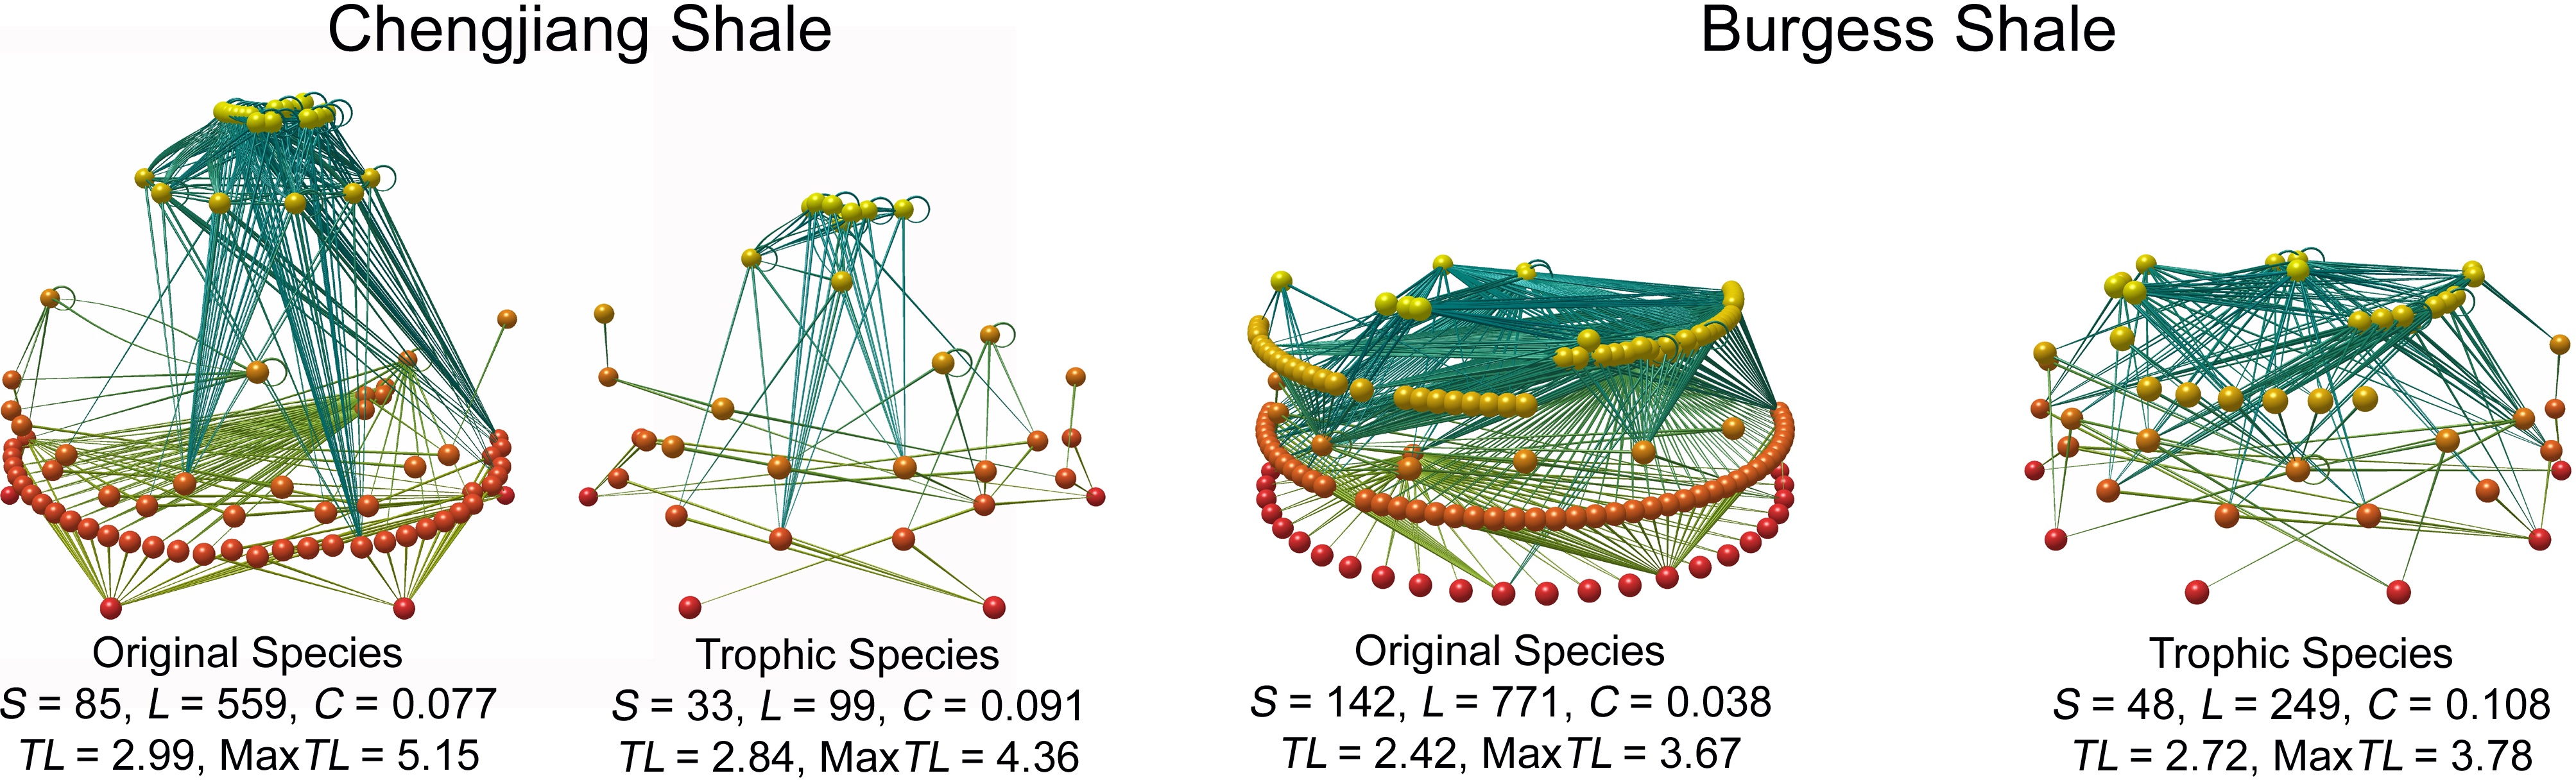
\includegraphics[scale=0.75]{Figures/INTRO_Chengjiang_and_Burgess_Shale_1.png}
\caption{Ejemplo de representación de cadenas tróficas como redes \cite{dunne2008compilation}. \small{\texttt{CC BY-SA 2.5}}.}
\label{fig:INTRO_Chengjiang_and_Burgess_Shale_1}
\end{figure}


\subsection{Redes mutualistas}

Las comunidades mutualistas se modelan como redes bipartitas, dirigidas y pesadas. Son bipartitas porque existen dos clases de nodos y las relaciones solo pueden establecerse entre especies de clases distintas. Los enlaces representan el beneficio que la especie $X$ de la clase $A$ aporta a la especie $Z$ de la clase $B$, por tanto son pesados \cite{barrat2004architecture}. La intensidad de este beneficio no es la misma que la que que recibe $X$ de $Z$, de manera que la red es dirigida. La figura \ref{fig:INTRO_bip_ficticia} muestra un diagrama bipartito de una comunidad mutualista. Para hacer más legibles los diagramas reales, la interacción entre dos especies se simplifica como un solo enlace no dirigido.

Una de las objeciones que pueden hacerse al modelado de las comunidades mutualistas como redes es su enfoque reduccionista. Tan solo se incluyen las interacciones positivas entre especies, pero como se ha explicado en el apartado \ref{TIPOS_DE_MUTUALISMO} la realidad puede ser mucho más rica. La simplificación es cierta. La red es una abstracción a la que podrían añadirse otros tipos de relación, posiblemente complicando el modelo hasta hacerlo inmanejable y mezclando los efectos del mutualismo con los de otros tipos de relación ecológica. En este punto conviene recordar la reflexión de George Box que abre la tesis. No hay modelos perfectos, pero algunos resultan útiles. A la vista de los resultados que ha producido esta forma de estudiar el mutualismo, es un modelo útil.

\begin{figure}[h!]
\centering
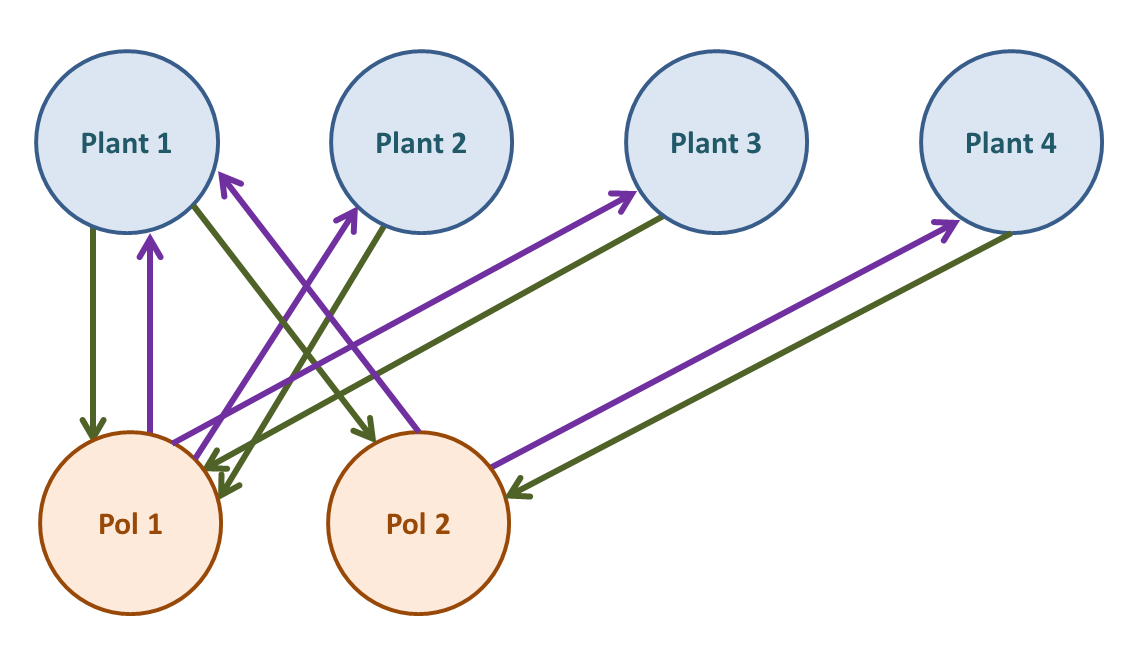
\includegraphics[scale=0.30]{Figures/INTRO_bip_ficticia.png}
\caption{Red mutualista ficticia con cuatro plantas y dos polinizadores}
\label{fig:INTRO_bip_ficticia}
\end{figure}

En su artículo seminal de 1987, Pedro Jordano aplicó de manera sistemática al mutualismo un enfoque de redes, utilizando las herramientas que se habían desarrollado para las cadenas tróficas.

\enquote{\itshape Entender como se distribuyen el número y la fuerza de los enlaces entre los distintos pares de especies es básico para entender la evolución del mutualismo en un determinado contexto} \cite{jordano1987patterns}.

El análisis partía de la \textit{matriz de interacción}. Las especies de una clase se disponen como filas y las de la otra como columnas, si existe interacción la casilla de la matriz está rellena (figura \ref{fig:VIS_matrix_SD_001}). Jordano observó que el número de interacciones crece con el tamaño de la red, como cabía esperar. La \textit{conectancia}, entendida como la fracción del número de enlaces existentes entre todos los posibles presentaba una gran heterogeneidad. A partir de la publicación de este artículo, la literatura sobre redes mutualistas ha conocido un crecimiento sostenido y vive en la actualidad un periodo de florecimiento \cite{gu2015emerging}.

Debido a las características de la relación mutualista, a lo largo de estos treinta años se han desarrollado modelos y medidas mucho más elaborados y específicos. Sin intención de hacer una revisión en profundidad, se describen a continuación los más relevantes para esta investigación.

\section{Dinámica de las comunidades mutualistas}

A pesar de su larga historia, hay aun muchos puntos abiertos en la investigación de la dinámica de poblaciones. Algunos de ellos fueron presentadas en el 125 aniversario de la revista {\em Science} hace ya una década  \cite{kennedy2005,pennisi2005,stokstad2005}. Por ejemplo, los mecanismos que dan origen y mantienen la biodiversidad en un ecosistema son objeto de investigación desde campos diversos por la comunidad científica \cite{williams2000,dunne2002biodiversity,olesen2007modularity,allesina2008,bascompte2009,saavedra2009,bastolla2009,fortuna2010nestedness,encinas2012}.  

El antecente más antiguo del estudio cuantitativo de las poblaciones se remonta a $1202$ cuando Leonardo Pisano (\textit{Fibonacci}), describió en su obra enciclopédica {\em Liber Abaci} la serie que sigue el crecimiento de una población de conejos \cite{sigler2002}. La teoría clásica de poblaciones, no obstante, se remonta a a $1798$ cuando Robert Malthus publicó {\em An Essay on the Principle of Population} \citep{malthus1798}. En dicha obra Malthus razonaba que el crecimiento de la población humana es proporcional al tamaño dado en un momento. Trasladándolo a una ecuación diferencial:
\begin{equation}
\frac{dN}{dt}=r_0\, N 
\label{eq:malthus}
\end{equation}
\noindent donde $N$ es el número de individuos y $r_0$ la {\em tasa intrínseca o vegetativa} de crecimiento de la polación, igual a la diferencia de las tasas de reproducción y defunciones cuando no hay migraciones.

El modelo malthusiano predice un crecimiento exponencial, así que si $r_0 > 0$ no tendría límite. En este modelo $r_0$ permanece constante a lo largo del proceso, sin tener en cuenta factores limitantes como la falta de alimentos o de espacio. En $1838$ Verhulst añadió un término adicional y llamó a su modelo modificado ecuación \emph{logística} \cite{verhulst1845}. La hipótesis de Verhulst es que la tasa de crecimiento debe reducirse conforme $N$ aumenta, hasta alcanzar un máximo. La forma matemática más simple de conseguirlo es haciendo que $r_0$ sea una función lineal de $N$: $ r_0 = r - \alpha N$, donde $r$ es la tasa intrínseca de crecimiento y $\alpha$ un coeficiente positivo de fricción que se interpreta como la competeción entre los individuos de la misma especie por los recursos que permiten su crecimiento y supervivencia. El modelo $r-\alpha$ de Verhulst es:
\begin{equation}
\frac{dN}{dt}=r \, N \,  - \alpha  \, N^2 
\label{eq:primitiveverhulst}
\end{equation}
El término $\alpha$ actúa como un freno biológico, que sitúa al sistema en un punto de equilibrio cuando la población alcanza un valor $ K = r / \alpha$, comúnmente denominado \emph{capcidad de carga}.

Sin embargo, la ecuación logística se conoce mucho más en la forma que Raymond Pearl introdujo en un libro de biometría en $1930$ (véase una excelente reseña histórica en \cite{mallet2012struggle}). En esta formulación, que se impuso en los libros de texto y en la literatura científica, la capacidad de carga aparece como un parámetro explícito de la ecuación y por ello se conoce como la forma $r-K$:

\begin{equation}
\frac{dN}{dt}=r \, N \, \left(1-\frac{N}{K}\right)
\label{pearl}
\end{equation}

La solución de esta ecuación es una curva sigmoide que crece asintóticamente hacia $K$. La fórmula de Pearl tiene algunos inconvenientes matemáticos importantes \citep{kuno1991some,gabriel2005paradoxes}. El más notable es que predice un absurdo crecimiento si la tasa $r$ es negativa pero la población inicial está por encima de la capacidad de carga. Este problema fue señalado por Richard Levins y en consecuencia de denomina \textit{paradoja de Levins}. Es importante señalarlo, porque todos los modelos de mutualismo se han derivado de la logística en la formulación de Pearl y por tanto arrastran este inconveniente.

Para solucionar el problema Levins propuso que $r$ debía ser siempre no negativa. Gabriel \emph{et al.} encontraron una solución más elegante usando la formulación original de Verhulst \cite{gabriel2005paradoxes}. La condición para que el sistema alcance la establidad es que el coeficiente $\alpha$ sea siempre positivo y la capacidad de carga se redefine como:

\begin{equation}
K_{\infty}=\lim_{t\rightarrow\infty}N(t),\; N(0)>0
\end{equation}

\noindent y entonces
\begin{equation*}
K_{\infty}=\left\{
\begin{array}{ll}
  \alpha / r = K, & \mathrm{si} \;\; \alpha > 0, \\ 0  & \mathrm{si} \;\; \alpha \le0 \\
  \end{array} \right.
\end{equation*}

Estos modelos primitivos de dinámica no incluían interacciones entre especies. Cuando varias de ellas comparten un mismo ecosistema aparece una compleja cadena de relaciones que puede modelarse como una red, como se mencionó en la introducción. En $1926$ Vito Volterra propuso un modelo de dos especies para explicar el comportamiento de algunos bancos de pesca en el Adriático \cite{volterra1926}. Las ecuaciones de Volterra describen las poblaciones de presa $N(t)$ y depredador $P(t)$ de la siguiente manera: 
\begin{align}
%\begin{split}
\displaystyle &\frac{dN}{dt}=N\, \left(a-b \,P\right) \nonumber\\
\displaystyle &\frac{dP}{dt}=P\, \left(c\, N-d\right) 
\label{myeq1}
%\end{split}
\end{align}
\noindent donde $a$, $b$, $c$ y $d$ son constantes positivas. En el modelo de Lotka-Volterra, como se conoce hoy, el crecimiento de la población de la presa está limitado por la población del derpedador y viceversa. Este par de ecuaciones tiene una solución oscilatoria.

El mutualismo, probablemente porque es una interacción menos abundante en la naturaleza, ha recibido menos atención históricamente, también desde el punto de vista matemático. El primer modelo fue propuesto por Richard May. Las ecuaciones de May representan una ecuación logística a la que se ha añadido un tercer término que representa el beneficio mutualista. Es la misma idea que la del modelo Lotka-Volterra, pero con un inconveninete analítico, las interacciones son siempre positivas, de manera que no hay oscilaciones y sí la posibilidad de un crecimimento ilimitado. El modelo de May se formaliza como:
\begin{align}
\frac{dN_1}{dt}=r_1 \,N_1\,\left(1-\frac{N_1}{K_1}\right)+r_1\, N_1\,\beta_{12}\, \frac{N_2}{K_1} \nonumber \\ 
\frac{dN_2}{dt}=r_2\, N_2\, \left(1-\frac{N_2}{K_2}\right)+r_2\, N_2\, \beta_{21} \, \frac{N_1}{K_2} 
\label{myeq2}
\end{align}
\noindent donde $N_1(N_2)$ es la población de la especie $1(2)$; $r_{1,2}$ es la tasa vegetativa de la población $1\, (2)$ y $K_1\, (K_2)$ la capacidad de carga. Este es el máximo que el entorno puede mantener en función de la disponibilidad de sustento y espacio. Por último, $\beta_{12}\,(\beta_{21})$ es el coeficiente que representa el beneficio mutualista para la especie $1\,(2)$ de su interacción con la $2\,(1)$. El principal inconveniente del modelo de May es que conduce a crecimiento ilimitado. No obstante, ha servido de inspiración para todos sus sucesores que incorporan términos adicionales para solucionar este problema.

Ha habido diferentes estrategias de ataque. Wright propuso un modelo de dos especies con saturación como resultado de las restricciones del \textit{handling time}, $T_H$, que corresponde al tiempo necesario para procesar los recursos (comida) producidos por la relación mutualista \cite{wright1989}. Esto dio lugar a la familia de modelos conocida como \textit{tipo II}:
\begin{align}
\frac{dN_1}{dt}=r_1\, N_1\, - \alpha_1 \, N_1^2+ \frac{a\, b\, N_1\,N_2}{1+ a\, N_2\,T_H} \nonumber\\
\frac{dN_2}{dt}=r_2\, N_2\, - \alpha_2 N_2^2 + \frac{a\,b\,N_1\,N_2}{1+a\, N_1\, T_H}
\label{eq_typeII}
\end{align}
\noindent donde $a$ es la tasa efectiva de búsqueda y $b$ un coeficiente que tiene en cuenta los encuentros entre individuos de las especies $1$ y $2$. La dinámica del modelo depende en gran medida del afinado de los parámetros, pero para un rango limitado de ellos muestra tres puntos fijos. Uno estable, que corresponde con la destrucción completa, otro también estable en máximos de población y un \textit{saddle} que separa las cuencas de atracción de los dos primeros. Usando un modelo tipo II, Bastolla demostró la importancia de la estructura de la red para minimizar la competencia entre especies y optimizar la biodiversidad \cite{bastolla2005,bastolla2009}. Los modelos de tipo II son, no obstante, difíciles de manejar analíticamente, debido a la forma en fracción del término mutualista. Hay otras alternativas recientes \cite{johnson2013} que proponen añadir términos adicionales al modelo tipo II, dificultando aun más el análisis.


\section{Cuestiones abiertas en el modelado del mutualismo}

Phasellus fermentum magna in augue gravida cursus. Cras sed pretium lorem. Pellentesque eget ornare odio. Proin accumsan, massa viverra cursus pharetra, ipsum nisi lobortis velit, a malesuada dolor lorem eu neque.

%----------------------------------------------------------------------------------------
%	ESTRUCTURA DE LA TESIS
%----------------------------------------------------------------------------------------

\section{Estructura de la tesis}
Morbi rutrum odio eget arcu adipiscing sodales. Aenean et purus a est pulvinar pellentesque. Cras in elit neque, quis varius elit. Phasellus fringilla, nibh eu tempus venenatis, dolor elit posuere quam, quis adipiscing urna leo nec orci. Sed nec nulla auctor odio aliquet consequat. Ut nec nulla in ante ullamcorper aliquam at sed dolor. Phasellus fermentum magna in augue gravida cursus. Cras sed pretium lorem. Pellentesque eget ornare odio. Proin accumsan, massa viverra cursus pharetra, ipsum nisi lobortis velit, a malesuada dolor lorem eu neque.
